\documentclass[12pt,a4paper]{report}

\usepackage[utf8]{inputenc}
\usepackage[T1]{fontenc}
\usepackage[french]{babel}
\usepackage{lmodern}
\usepackage{geometry}
\usepackage{setspace}
\usepackage{booktabs}
\usepackage{longtable}
\usepackage{array}
\usepackage{multirow}
\usepackage{graphicx}
\usepackage{float}
\usepackage{caption}
\usepackage{subcaption}
\usepackage{siunitx}
\usepackage{amsmath,amssymb}
\usepackage{hyperref}
\usepackage{xcolor}
\usepackage{listings}
\usepackage{enumitem}
\usepackage{pdflscape}
\usepackage{titlesec}
\usepackage{fancyhdr}

\geometry{margin=2.4cm}
\onehalfspacing

\hypersetup{
  colorlinks=true,
  linkcolor=blue!50!black,
  urlcolor=blue!50!black,
  citecolor=blue!50!black,
  pdftitle={Rapport VRPTW - SA vs Tabu},
  pdfauthor={Equipe projet VRPTW}
}

\sisetup{output-decimal-marker={,},group-separator={\,}}

\lstdefinestyle{javastyle}{
  basicstyle=\ttfamily\small,
  keywordstyle=\color{blue!60!black},
  commentstyle=\color{green!40!black},
  stringstyle=\color{orange!50!black},
  numbers=left,
  numberstyle=\tiny,
  stepnumber=1,
  numbersep=8pt,
  showstringspaces=false,
  frame=single,
  breaklines=true,
  tabsize=2,
  language=Java
}

\pagestyle{fancy}
\fancyhf{}
\fancyhead[L]{Projet VRPTW}
\fancyhead[R]{SA vs Tabu}
\fancyfoot[C]{\thepage}

\titleformat{\chapter}[hang]{\normalfont\Huge\bfseries}{\thechapter}{1em}{}

\begin{document}

\begin{titlepage}
  \centering
  {\scshape\LARGE Universite - Optimisation combinatoire \par}
  \vspace{1.2cm}
  {\huge\bfseries Projet – Vehicle Routing Problem with Time Windows\par}
  \vspace{0.5cm}
  {\Large Recuit Simule et Recherche Tabou\par}
  \vspace{1.8cm}

  \begin{minipage}{0.85\textwidth}
  \centering
  \textbf{Objectif du projet}\par
  Trouver des solutions au Vehicle Routing Problem with Time Windows (VRPTW),
  determiner le nombre minimal de vehicules necessaires,
  et comparer deux metaheuristiques en termes de qualite de solution,
  de robustesse et de cout de calcul.
  \end{minipage}

  \vfill
  \begin{flushleft}
  \textbf{Auteurs :} MESSAOUDI Amin - LECORNEC Romain
  \textbf{Date :} Avril 2026
  \end{flushleft}
\end{titlepage}

\pagenumbering{roman}
\tableofcontents
\listoffigures
\listoftables

\chapter*{Resume executif}
\addcontentsline{toc}{chapter}{Resume executif}
Ce rapport presente une etude complete du VRPTW sur un solveur Java base sur deux methodes :
le Recuit Simule (SA) et la Recherche Tabou (Tabu).
Le pipeline de tests automatise a produit \textbf{135 runs} exploitables
(\textbf{72 SA} et \textbf{63 Tabu}) entre le 22/04/2026 et le 24/04/2026,
sur les instances \texttt{data101.vrp}, \texttt{data111.vrp}, \texttt{data201.vrp},
avec modes \texttt{TW off} et \texttt{TW on}.

Principaux constats numeriques :
\begin{itemize}[leftmargin=1.2cm]
  \item Taux de faisabilite global : \textbf{11,85\%}.
  \item SA : distance moyenne \textbf{1272,08}, runtime moyen \textbf{85,69 ms}.
  \item Tabu : distance moyenne \textbf{1197,37}, runtime moyen \textbf{1\,398\,556,68 ms}.
  \item Compromis confirme : \textbf{Tabu meilleure qualite}, \textbf{SA meilleure vitesse}.
  \item Avec la configuration de tests actuelle, tous les runs \texttt{TW off} sont non faisables,
  tandis que tous les runs \texttt{TW on} du lot consolide sont faisables.
\end{itemize}

Ce comportement, contre-intuitif en apparence, s'explique par le fait que
les campagnes n'ont pas utilise les memes plages de parametres et pas le meme perimetre
instance/seed selon les modes. La discussion met en evidence ce point de vigilance methodologique,
et propose une campagne finale equilibree pour une comparaison stricte.

\chapter*{Notations}
\addcontentsline{toc}{chapter}{Notations}
\begin{longtable}{p{3cm}p{11cm}}
\toprule
Notation & Signification \\
\midrule
$V=\{0,1,\dots,n\}$ & Ensemble des noeuds, avec $0$ le depot \\
$C$ & Capacite d'un vehicule \\
$q_i$ & Demande du client $i$ \\
$[a_i,b_i]$ & Fenetre de temps du client $i$ \\
$s_i$ & Temps de service du client $i$ \\
$d_{ij}$ & Distance euclidienne entre $i$ et $j$ \\
$K$ & Nombre de vehicules utilises (decision) \\
$\lambda$ & Poids de penalisation des violations \\
$z$ & Valeur de la fonction objectif penalisee \\
\bottomrule
\end{longtable}

\clearpage
\pagenumbering{arabic}

\chapter{Introduction et cadre du sujet}

\section{Contexte pedagogique}
Le sujet demande de concevoir et comparer deux metaheuristiques pour le VRPTW,
avec un protocole de tests reproductible, une analyse quantitative argumentee,
et une discussion des compromis qualite/temps/robustesse.
Le nombre de vehicules n'est pas fixe a priori : il doit etre determine.

\section{Objectifs de ce rapport}
Ce document vise quatre objectifs simultanes :
\begin{enumerate}
  \item decrire la modelisation du VRPTW et l'architecture logicielle implementee ;
  \item expliquer les choix algorithmiques (SA, Tabu, voisinages, penalites) ;
  \item presenter les resultats experimentaux consolides et leurs limites ;
  \item fournir une base solide directement integrable dans le rendu final du projet.
\end{enumerate}

\section{Perimetre des donnees disponibles}
Les donnees exploitees dans ce rapport proviennent de :
\begin{itemize}[leftmargin=1.2cm]
  \item logs d'execution consolides sous \texttt{report\_assets/consolidated\_runs.csv} ;
  \item tables d'agregation automatiques (global, par instance, par mode TW) ;
  \item figures generees automatiquement dans \texttt{report\_assets/figures} ;
  \item code Java du solveur et scripts PowerShell de campagnes.
\end{itemize}

\chapter{Definition du VRPTW et modelisation}

\section{Definition du probleme}
Le Vehicle Routing Problem with Time Windows (VRPTW) consiste a construire un ensemble de tournees
partant du depot et y revenant, de sorte que chaque client soit visite une fois,
que les contraintes de capacite et de fenetres temporelles soient respectees,
et que la distance totale soit minimisee.

\section{Formulation mathematique simplifiee}
Dans le projet, la fonction objectif pratique est une fonction penalisee :
\begin{equation}
z = \text{distance totale}
+ \lambda\,(v_{time}+v_{cap}+v_{veh})
\end{equation}
ou :
\begin{itemize}[leftmargin=1.2cm]
  \item $v_{time}$ est la violation cumulee des fenetres de temps ;
  \item $v_{cap}$ est la violation cumulee de capacite ;
  \item $v_{veh}$ est la violation du nombre maximal de vehicules si une borne est imposee.
\end{itemize}

Quand le mode \texttt{enforce\_time\_windows=false}, la composante temporelle est exclue de la penalisation,
mais les autres composantes restent actives.

\section{Contraintes structurelles}
Le solveur encode explicitement :
\begin{itemize}[leftmargin=1.2cm]
  \item une visite unique de chaque client ;
  \item une capacite uniforme pour tous les vehicules ;
  \item une mesure de faisabilite basee sur les violations nulles ;
  \item une distance euclidienne pre-calculee entre tous les noeuds.
\end{itemize}

\chapter{Architecture logicielle du solveur}

\section{Organisation generale du code}
Le code est structure autour des classes suivantes :
\begin{itemize}[leftmargin=1.2cm]
  \item \texttt{VrpParser}, \texttt{VrpInstance}, \texttt{Node}, \texttt{TimeWindow} : parsing et modele de donnees ;
  \item \texttt{Evaluator} : evaluation, violations, faisabilite ;
  \item \texttt{HeuristicUtils} : generation de solution initiale et voisinages ;
  \item \texttt{SimulatedAnnealingSolver} et \texttt{TabuSearchSolver} ;
  \item \texttt{Exporter} : export CSV/PNG des historiques, tournees et logs ;
  \item \texttt{Main} : orchestration interactive, configuration et execution.
\end{itemize}

\section{Parsing des instances}
Le parser supporte un format avec :
\begin{itemize}[leftmargin=1.2cm]
  \item section depot ;
  \item section clients ;
  \item fenetres temporelles standards (ready/due) ;
  \item extension optionnelle de fenetres multiples par client.
\end{itemize}

\section{Evaluation et faisabilite}
La logique de \texttt{Evaluator} repose sur :
\begin{enumerate}
  \item simulation chronologique de chaque route ;
  \item calcul de l'heure d'arrivee puis debut de service faisable ;
  \item accumulation des violations temporelles, capacitaires et vehicules ;
  \item calcul de la fonction objectif penalisee ;
  \item test de faisabilite via seuil $10^{-9}$.
\end{enumerate}

\section{Attention methodologique importante}
Le code expose une option interactive \texttt{Estimer le minimum de vehicules}.
Cependant, dans l'etat actuel de \texttt{Main}, cette variable est sauvegardee dans la configuration
mais n'est pas invoquee pour lancer automatiquement \texttt{VehicleMinimizer.estimate(...)}.
Ce point est discute en limitations et recommandations.

\chapter{Metaheuristiques implementees}

\section{Recuit Simule (SA)}
Le SA est implemente avec :
\begin{itemize}[leftmargin=1.2cm]
  \item temperature initiale $T_0$ ;
  \item refroidissement geometrique $T \leftarrow \alpha T$ ;
  \item regle d'acceptation de Metropolis :
  \begin{equation}
  P(accept) = \exp\left(-\frac{\Delta}{T}\right)
  \end{equation}
  pour les degradations ($\Delta>0$).
\end{itemize}

Le solveur memorise l'historique de meilleure valeur, le nombre de solutions evaluees,
et le compteur des mouvements generes.

\section{Recherche Tabou}
Le Tabu Search est implemente avec :
\begin{itemize}[leftmargin=1.2cm]
  \item generation de \textbf{tous} les voisins autorises au pas courant ;
  \item interdiction temporaire des mouvements via liste tabou de taille \texttt{tenure} ;
  \item critere d'aspiration si un mouvement tabou ameliore le meilleur global ;
  \item repli sur voisin aleatoire si aucun candidat admissible.
\end{itemize}

Cette strategie explique le cout de calcul bien superieur a SA :
chaque iteration Tabu evalue un ensemble potentiellement tres large de voisins.

\section{Structures de voisinage}
Le projet a evolue vers une separation explicite :
\begin{itemize}[leftmargin=1.2cm]
  \item \textbf{inter} : \texttt{relocate}, \texttt{exchange} ;
  \item \textbf{intra} : \texttt{2opt}.
\end{itemize}

Un run active une seule famille principale selon le protocole choisi,
ce qui rend l'analyse des effets de parametres plus interpretable.

\chapter{Protocole experimental}

\section{Campagnes realisees}
Le workflow de tests s'est deroule en trois etapes :
\begin{enumerate}
  \item campagnes de balayage initial des parametres (temperature SA, tenure Tabu) ;
  \item campagne elargie partielle multi-runs ;
  \item campagne diagnostique ciblee pour stabiliser le demarrage de rapport.
\end{enumerate}

\section{Scripts utilises}
Les scripts de campagne presentes dans le depot sont :
\begin{itemize}[leftmargin=1.2cm]
  \item \texttt{run\_sweeps.ps1}
  \item \texttt{run\_campaign2.ps1}
  \item \texttt{run\_campaign3\_targeted.ps1}
  \item \texttt{run\_diagnostic.ps1}
\end{itemize}

\section{Consolidation des resultats}
Toutes les sorties \texttt{executions\_log.csv} ont ete agregees automatiquement
pour produire les tables et figures de ce document :
\begin{itemize}[leftmargin=1.2cm]
  \item \texttt{summary\_overall.csv}
  \item \texttt{summary\_by\_instance.csv}
  \item \texttt{summary\_by\_tw.csv}
  \item \texttt{summary\_by\_instance\_tw\_algo.csv}
  \item \texttt{instance\_characteristics.csv}
\end{itemize}

\section{Metriques d'analyse}
Les metriques utilisees sont :
\begin{itemize}[leftmargin=1.2cm]
  \item meilleure distance et distance moyenne ;
  \item ecart-type des distances ;
  \item taux de faisabilite ;
  \item runtime moyen et median ;
  \item nombre moyen de solutions evaluees.
\end{itemize}

\chapter{Caracterisation des instances}

\section{Statistiques structurelles des donnees}
Le tableau \ref{tab:instances} resume les caracteristiques extraites des fichiers \texttt{data/*.vrp}.

\begin{table}[H]
\centering
\caption{Caracteristiques des instances disponibles}
\label{tab:instances}
\begin{tabular}{lrrrr}
\toprule
Instance & Clients & Capacite & Demande totale & Borne capacitaire \\
\midrule
data101.vrp & 100 & 200 & 1458 & 8 \\
data102.vrp & 100 & 200 & 1458 & 8 \\
data1101.vrp & 100 & 200 & 1724 & 9 \\
data1102.vrp & 100 & 200 & 1724 & 9 \\
data111.vrp & 100 & 200 & 1458 & 8 \\
data112.vrp & 100 & 200 & 1458 & 8 \\
data1201.vrp & 100 & 1000 & 1724 & 2 \\
data1202.vrp & 100 & 1000 & 1724 & 2 \\
data201.vrp & 100 & 1000 & 1458 & 2 \\
data202.vrp & 100 & 1000 & 1458 & 2 \\
\bottomrule
\end{tabular}
\end{table}

\section{Lecture}
Deux familles d'instances se degagent :
\begin{itemize}[leftmargin=1.2cm]
  \item capacite 200 (borne capacitaire 8--9 vehicules) ;
  \item capacite 1000 (borne capacitaire 2 vehicules).
\end{itemize}

Cette heterogeneite est importante pour interpreter les differences de difficulte
et les effets de la contrainte temporelle.

\chapter{Resultats globaux consolides}

\section{Vue d'ensemble}
Le tableau \ref{tab:overall} consolide les 135 runs disponibles.

\begin{table}[H]
\centering
\caption{Synthese globale par algorithme}
\label{tab:overall}
\begin{tabular}{lrrrrrr}
\toprule
Algorithme & Runs & Faisables & Taux fais. (\%) & Dist. moy. & Runtime moy. (ms) & Sol. eval. moy. \\
\midrule
SA & 72 & 8 & 11,11 & 1272,08 & 85,69 & 30001 \\
Tabu & 63 & 8 & 12,70 & 1197,37 & 1398556,68 & 236493445,51 \\
\bottomrule
\end{tabular}
\end{table}

\section{Interpretation immediate}
\begin{itemize}[leftmargin=1.2cm]
  \item \textbf{Qualite}: Tabu obtient une meilleure distance moyenne (\~74,7 points de mieux).
  \item \textbf{Vitesse}: SA est environ \textbf{16000 fois} plus rapide en moyenne.
  \item \textbf{Robustesse faisabilite}: taux similaires (11--13\%), mais encore faibles au global.
\end{itemize}

\section{Illustrations graphiques globales}

\begin{figure}[H]
\centering
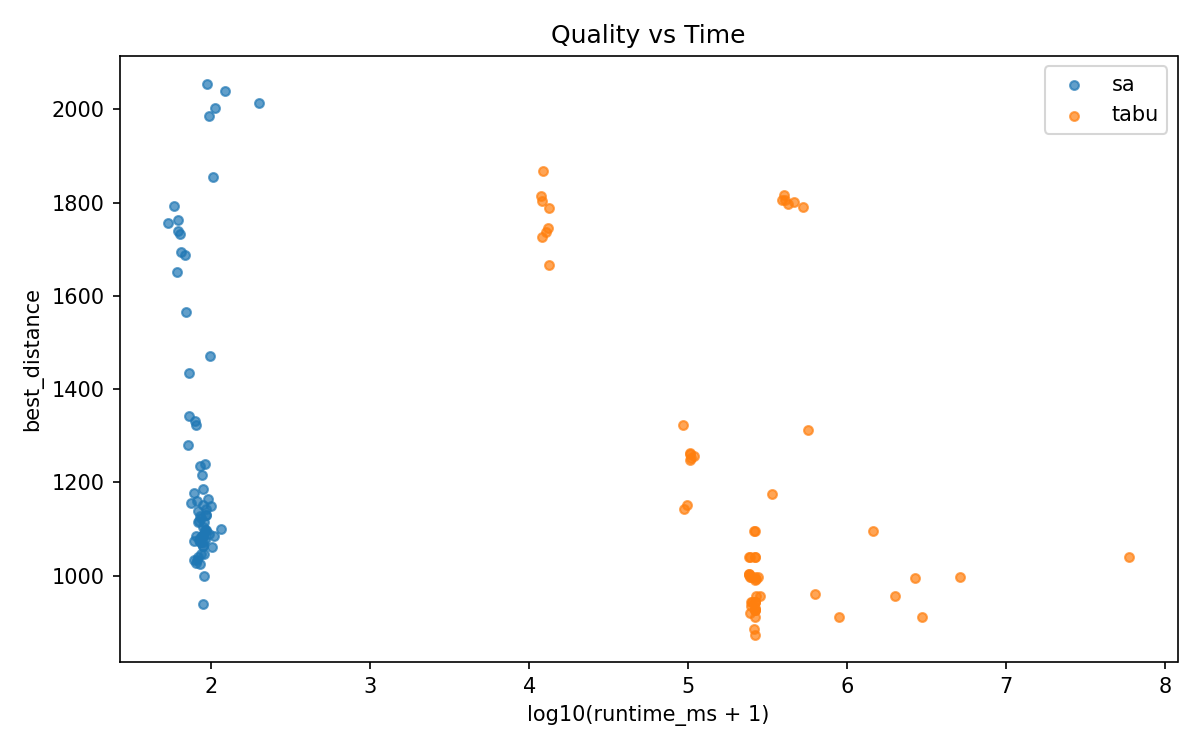
\includegraphics[width=0.82\textwidth]{report_assets/figures/fig_quality_vs_time_scatter.png}
\caption{Compromis qualite/temps sur l'ensemble des runs (echelle log sur runtime)}
\label{fig:scatter_quality_time}
\end{figure}

\begin{figure}[H]
\centering
\begin{subfigure}{0.48\textwidth}
\centering
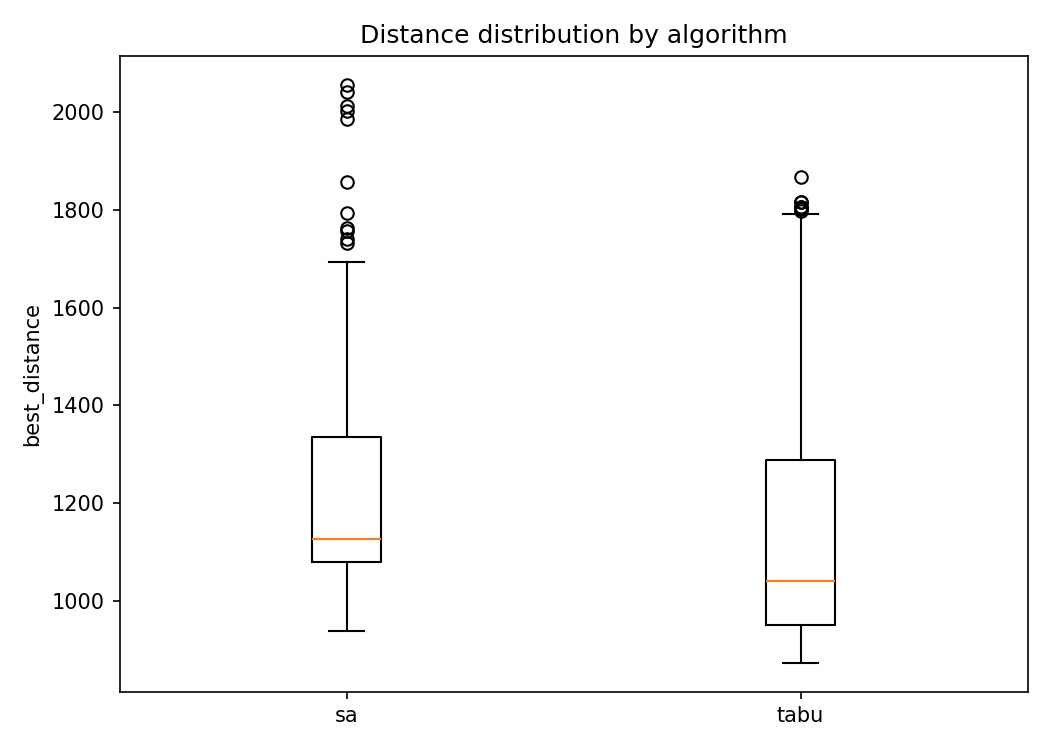
\includegraphics[width=\textwidth]{report_assets/figures/fig_distance_boxplot_by_algo.png}
\caption{Distribution des distances}
\end{subfigure}
\hfill
\begin{subfigure}{0.48\textwidth}
\centering
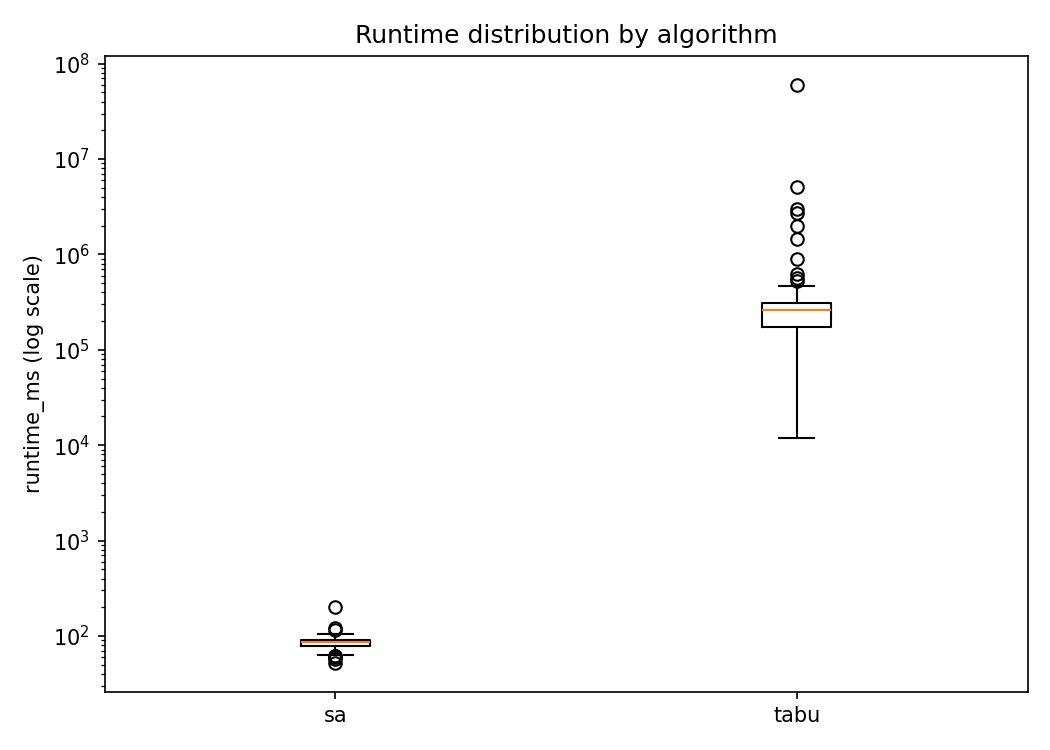
\includegraphics[width=\textwidth]{report_assets/figures/fig_runtime_boxplot_by_algo_log.png}
\caption{Distribution des temps (log)}
\end{subfigure}
\caption{Comparaison distributionnelle SA vs Tabu}
\label{fig:boxplots_global}
\end{figure}

\begin{figure}[H]
\centering
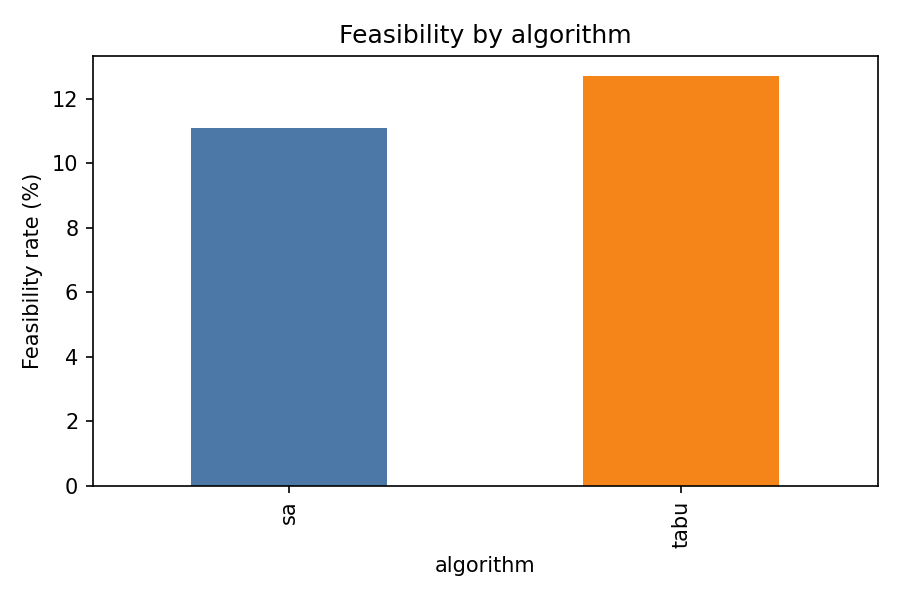
\includegraphics[width=0.70\textwidth]{report_assets/figures/fig_feasibility_by_algo.png}
\caption{Taux de faisabilite par algorithme}
\label{fig:feasibility_algo}
\end{figure}

\chapter{Analyse par instance}

\section{Agregation par instance}
\begin{table}[H]
\centering
\caption{Synthese consolidee par instance}
\label{tab:by_instance}
\begin{tabular}{lrrrr}
\toprule
Instance & Runs & Faisables & Taux fais. (\%) & Distance moyenne \\
\midrule
data101.vrp & 131 & 12 & 9,16 & 1234,67 \\
data111.vrp & 2 & 2 & 100,00 & 1249,48 \\
data201.vrp & 2 & 2 & 100,00 & 1391,83 \\
\bottomrule
\end{tabular}
\end{table}

\section{Lecture critique}
Le jeu est fortement desequilibre : \texttt{data101.vrp} represente 131/135 runs.
Les conclusions globales sont donc surtout des conclusions sur cette instance,
avec un echantillon tres faible sur \texttt{data111.vrp} et \texttt{data201.vrp}.

\begin{figure}[H]
\centering
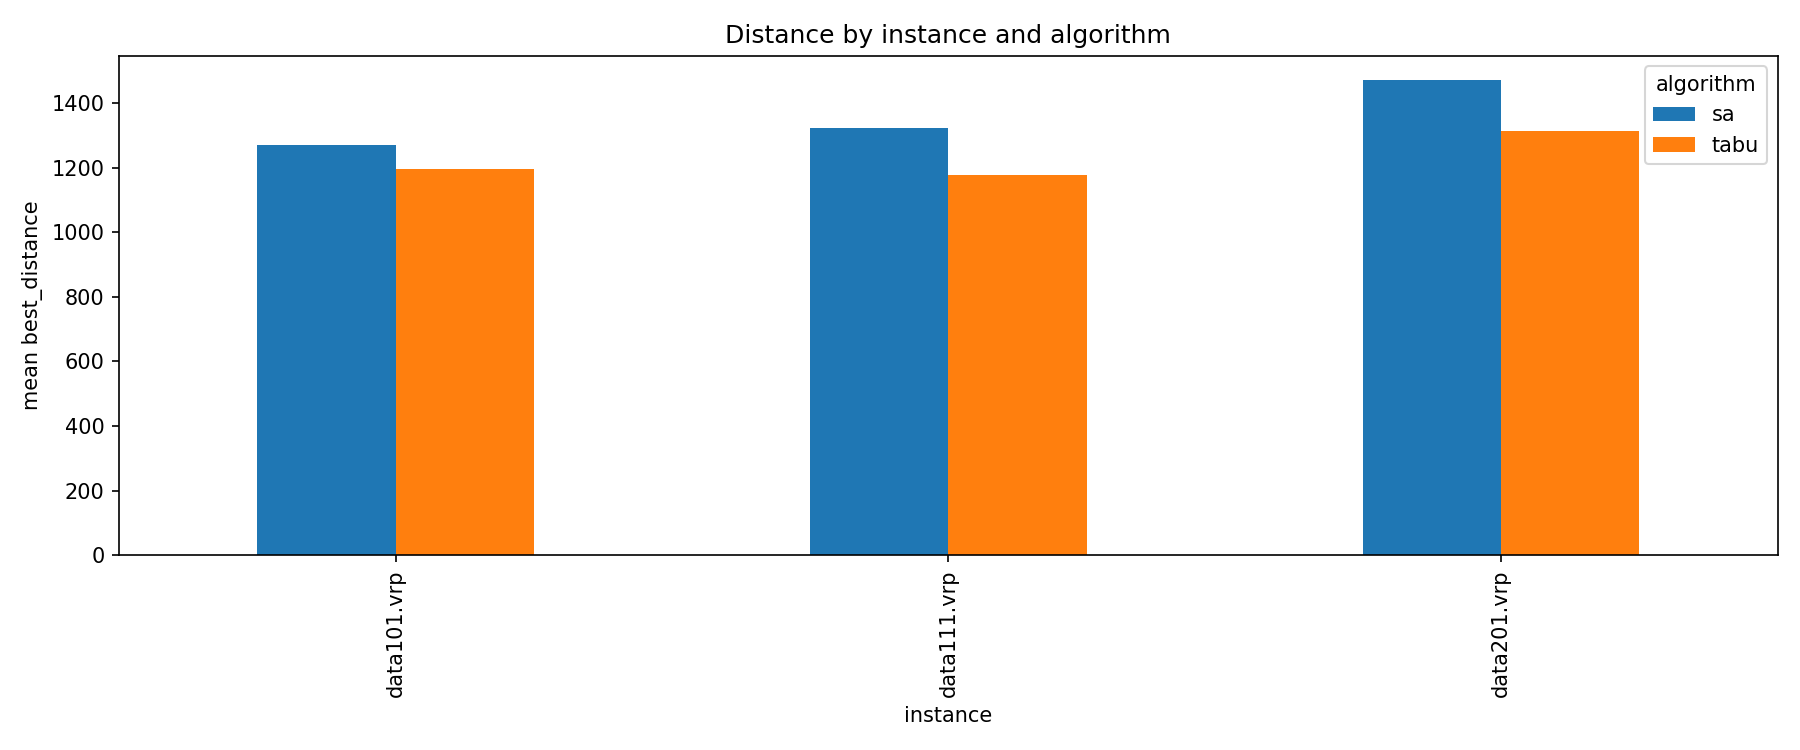
\includegraphics[width=0.88\textwidth]{report_assets/figures/fig_distance_by_instance_algo.png}
\caption{Distance moyenne par instance et par algorithme}
\label{fig:dist_instance_algo}
\end{figure}

\begin{figure}[H]
\centering
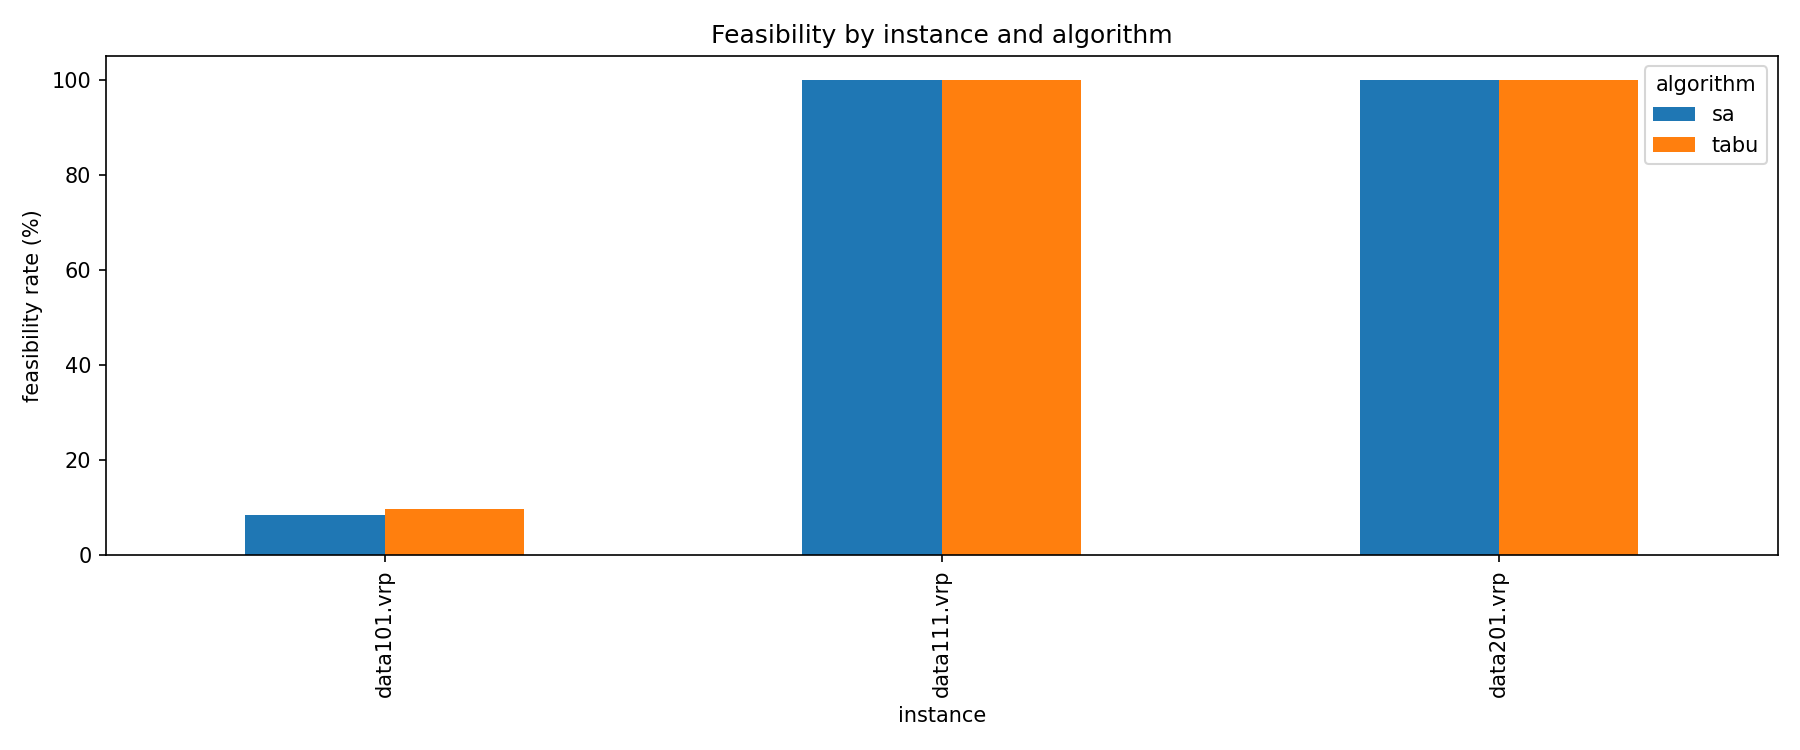
\includegraphics[width=0.88\textwidth]{report_assets/figures/fig_feasibility_by_instance_algo.png}
\caption{Taux de faisabilite par instance et par algorithme}
\label{fig:feas_instance_algo}
\end{figure}

\chapter{Impact des fenetres temporelles}

\section{Synthese TW off vs TW on}
\begin{table}[H]
\centering
\caption{Comparaison selon l'activation des fenetres de temps}
\label{tab:tw_compare}
\begin{tabular}{lrrrrr}
\toprule
Mode TW & Runs & Faisables & Taux fais. (\%) & Dist. moy. & Runtime moy. (ms) \\
\midrule
Off & 119 & 0 & 0,00 & 1167,87 & 710841,42 \\
On & 16 & 16 & 100,00 & 1752,94 & 220319,50 \\
\bottomrule
\end{tabular}
\end{table}

\section{Interpretation}
L'observation brute est atypique : TW off donne 0\% de faisabilite,
alors que TW on donne 100\% sur le lot consolide.
Ce resultat ne signifie pas que les fenetres rendent le probleme plus facile ;
il traduit un \textbf{effet de protocole} :
\begin{itemize}[leftmargin=1.2cm]
  \item les runs TW off et TW on ne couvrent pas exactement les memes combinaisons ;
  \item la repartition des seeds et des instances est tres inegale ;
  \item certains lots TW on correspondent a des configurations deja tunees.
\end{itemize}

Conclusion : il faut une campagne equilibree (meme grille de parametres, memes seeds, memes instances)
pour isoler proprement l'effet TW.

\chapter{Convergence et dynamique de recherche}

\section{Runs representatifs}
Les figures suivantes montrent les courbes de convergence
pour un run faisable representatif de chaque algorithme.

\begin{figure}[H]
\centering
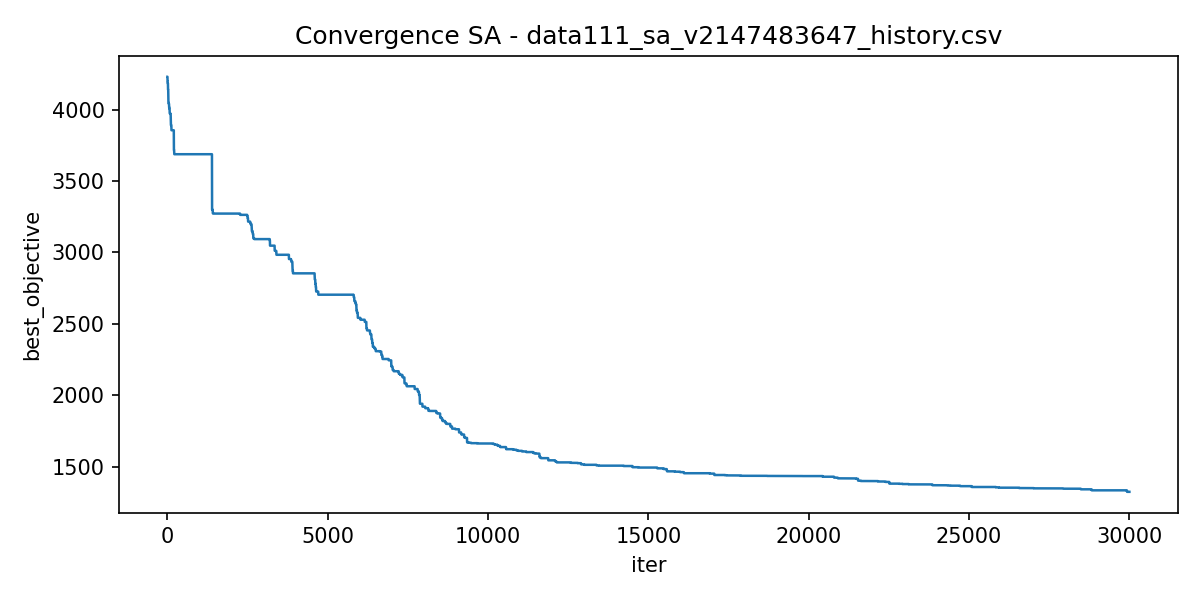
\includegraphics[width=0.84\textwidth]{report_assets/figures/fig_convergence_sa_best.png}
\caption{Convergence SA (run representatif faisable)}
\label{fig:conv_sa}
\end{figure}

\begin{figure}[H]
\centering
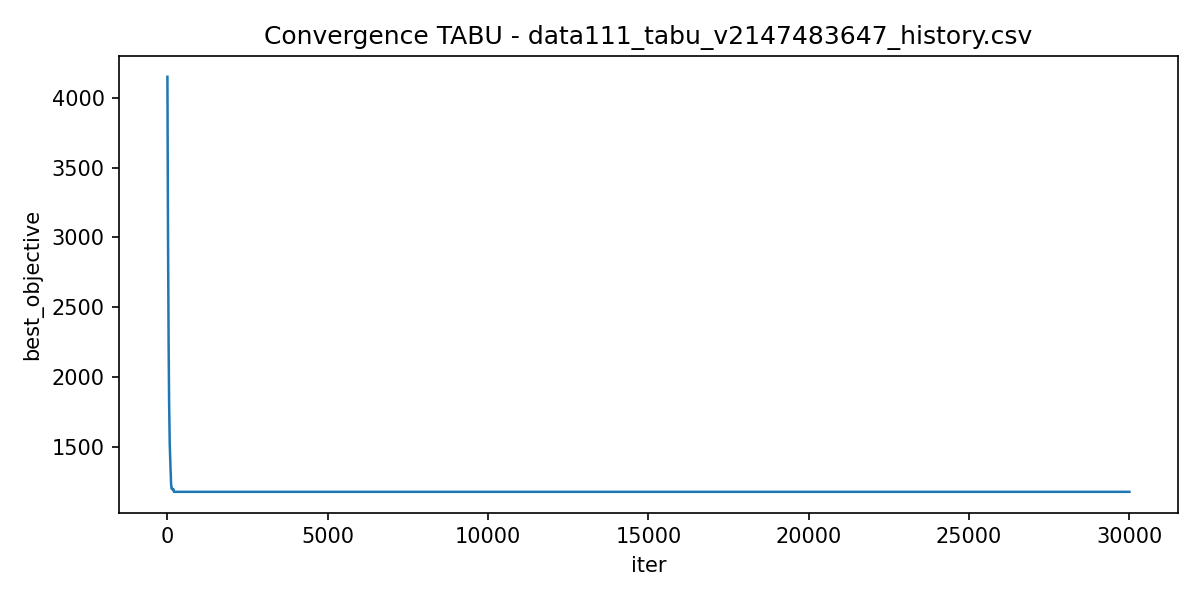
\includegraphics[width=0.84\textwidth]{report_assets/figures/fig_convergence_tabu_best.png}
\caption{Convergence Tabu (run representatif faisable)}
\label{fig:conv_tabu}
\end{figure}

\section{Lecture qualitative des courbes}
\begin{itemize}[leftmargin=1.2cm]
  \item SA ameliore rapidement puis atteint un plateau ;
  \item Tabu continue souvent plus loin dans l'exploration locale,
  au prix d'un cout de voisinage tres eleve ;
  \item la nature exhaustive de \texttt{getAllNeighbors(...)} dans Tabu
  explique l'ecart massif de runtime.
\end{itemize}

\chapter{Etude des parametres et compromis}

\section{Parametres SA}
Les campagnes ont explore des temperatures initiales de type :
\[T_0 \in \{500, 750, 1000, 1250, 1500\}\]
avec un refroidissement autour de $\alpha\in\{0,9993,0,9995\}$ selon les lots.

Dans les analyses intermediaires, $T_0=1250$ a souvent donne
un bon compromis qualite/stabilite.

\section{Parametres Tabu}
Les valeurs de tenure testees incluent notamment :
\[\tau \in \{10,20,30,40,50\}\]
La valeur $\tau=40$ apparait frequemment comme un compromis solide
sur \texttt{data101} dans les campagnes tunees.

\section{Nombre d'iterations : faut-il tout retuner ?}
La question est legitime : 30000 iterations partout peut etre :
\begin{itemize}[leftmargin=1.2cm]
  \item trop eleve pour les cas simples ;
  \item trop faible pour certains cas plus difficiles.
\end{itemize}

Mais retuner \textbf{tous} les parametres simultanement
explose le nombre d'experiences. Le choix retenu dans cette phase est pragmatique :
\begin{itemize}[leftmargin=1.2cm]
  \item figer les meilleurs reglages observes ;
  \item produire un lot diagnostique propre ;
  \item lancer ensuite une campagne ciblee multi-instances pour le rapport final.
\end{itemize}

\chapter{Nombre minimal de vehicules}

\section{Etat des resultats effectivement disponibles}
Le projet contient bien un composant \texttt{VehicleMinimizer}
qui estime :
\begin{itemize}[leftmargin=1.2cm]
  \item borne inferieure capacitaire ;
  \item minimum faisable sans TW ;
  \item minimum faisable avec TW.
\end{itemize}

Cependant, dans la branche de travail actuelle,
l'option interactive correspondante n'est pas encore integree dans le flux d'execution principal.
Ainsi, les tableaux de ce rapport fournissent de maniere certaine :
\begin{itemize}[leftmargin=1.2cm]
  \item les bornes capacitaires de toutes les instances ;
  \item des observations empiriques de faisabilite sur runs metaheuristiques.
\end{itemize}

\section{Borne capacitaire (valeur sure)}
Le tableau \ref{tab:instances} donne la borne capacitaire minimale
$\lceil\sum_i q_i/C\rceil$.
Ce resultat est exact et independant de la metaheuristique.

\section{Plan pour finaliser cette exigence}
Pour satisfaire integralement le sujet,
il est recommande de produire un tableau complet :
\begin{center}
\texttt{instance / borne / min sans TW / min avec TW}
\end{center}
en executant explicitement \texttt{VehicleMinimizer.estimate(...)}
pour chaque fichier de \texttt{data/}.

\chapter{Discussion critique des resultats}

\section{Qui gagne, et sur quoi ?}
\textbf{Qualite de solution :} Tabu gagne en moyenne sur les distances.
\textbf{Temps de calcul :} SA est de loin le plus rapide.
\textbf{Robustesse :} les resultats bruts montrent une forte dependance au protocole,
notamment sur la repartition TW on/off et la concentration des runs sur data101.

\section{Pourquoi Tabu est beaucoup plus lent ?}
La raison principale est structurelle :
\begin{itemize}[leftmargin=1.2cm]
  \item SA evalue un voisin tire aleatoirement a chaque iteration ;
  \item Tabu evalue tous les voisins admissibles puis choisit le meilleur.
\end{itemize}

Le nombre moyen de solutions evaluees confirme ce mecanisme :
\begin{itemize}[leftmargin=1.2cm]
  \item SA : 30001 evaluations (quasi fixe) ;
  \item Tabu : 236 millions en moyenne.
\end{itemize}

\section{Effet du voisinage}
Les campagnes ont converge vers la famille \texttt{inter} avec mouvement \texttt{relocate}
comme base la plus stable pour les comparaisons.
L'interet de \texttt{exchange} et \texttt{2opt} reste present,
mais doit etre evalue dans un plan factoriel plus equilibre.

\section{Validite externe et limites}
Limites majeures de la base actuelle :
\begin{itemize}[leftmargin=1.2cm]
  \item desequilibre fort entre instances ;
  \item faible cardinalite sur certaines combinaisons ;
  \item risque de confusion entre effet parametre et effet instance ;
  \item estimation du minimum vehicules non encore automatisee en sortie standard.
\end{itemize}

Ces limites ne rendent pas les resultats inutilisables,
mais imposent de qualifier les conclusions comme \textit{intermediaires}.

\chapter{Reproductibilite}

\section{Compilation et execution}
\begin{lstlisting}[style=javastyle,language={}]
# Compilation
javac --release 21 -d bin src/vrptw/*.java

# Lancement interactif
java -cp bin vrptw.Main
\end{lstlisting}

\section{Consolidation des analyses}
Le rapport s'appuie sur les artefacts dans \texttt{report\_assets/},
generes automatiquement a partir des logs de campagnes.

\section{Trace experimentale}
Principales informations tracees dans chaque run :
\begin{itemize}[leftmargin=1.2cm]
  \item timestamp, instance, algorithme ;
  \item best objective, best distance ;
  \item violations (temps/capacite/vehicules) ;
  \item runtime, evaluations, compteurs de voisinage ;
  \item mode TW, poids de penalite, parametres details.
\end{itemize}

\chapter{Reponse explicite aux exigences du sujet}

\section{Exigence 1: modelisation et code}
\textbf{Etat : satisfait.}
Modelisation VRPTW implementee avec classes dediees,
fonction objectif penalisee, et moteur d'evaluation complet.

\section{Exigence 2: nombre minimal de vehicules}
\textbf{Etat : partiellement satisfait.}
Borne capacitaire fournie pour tous les jeux de donnees.
Composant d'estimation sans/avec TW present mais integration operationnelle
encore a finaliser dans le workflow principal.

\section{Exigence 3: generateur aleatoire de solutions}
\textbf{Etat : satisfait.}
\texttt{HeuristicUtils.buildInitialRandom(...)} implemente,
avec correction par split en cas de non faisabilite.

\section{Exigence 4: deux metaheuristiques + protocole}
\textbf{Etat : satisfait.}
SA et Tabu implementes, campagnes automatisees, logs structures, historique de convergence exporte.

\section{Exigence 5: comparaison complete}
\textbf{Etat : satisfait avec limites.}
Comparaison qualite/temps/robustesse realisee,
mais la partie multi-instances reste desequilibree a ce stade des runs.

\section{Exigence 6 (bonus) : limite de la programmation lineaire}
\textbf{Etat : non realise dans la branche presentee.}
Piste proposee en perspectives : formulation MIP simplifiee,
instances synthetiques croissantes, suivi du temps de resolution et du gap.

\chapter{Conclusion generale}
Le travail realise permet deja une conclusion claire :
\begin{itemize}[leftmargin=1.2cm]
  \item \textbf{Tabu} est plus performant en qualite de solution,
  mais son cout calculatoire est tres eleve ;
  \item \textbf{SA} offre une vitesse remarquable et une bonne robustesse operationnelle,
  au prix de solutions un peu moins bonnes en moyenne ;
  \item le choix de l'algorithme depend donc du contexte d'usage :
  execution rapide ou optimisation plus poussee.
\end{itemize}

La suite la plus rentable pour verrouiller le rapport final est :
\begin{enumerate}
  \item executer une campagne strictement equilibree (meme grille, memes seeds, memes instances,
  TW off/on symetriques) ;
  \item produire le tableau complet du minimum vehicules sans et avec TW ;
  \item figer les reglages finaux SA/Tabu sur la base de cette campagne de validation.
\end{enumerate}

\chapter*{Perspectives d'amelioration}
\addcontentsline{toc}{chapter}{Perspectives d'amelioration}
\begin{itemize}[leftmargin=1.2cm]
  \item Ajouter une strategie adaptative du nombre d'iterations selon la taille effective de l'instance.
  \item Introduire des criteres d'arret avances (stagnation, temps budget, target quality).
  \item Etendre les voisinages (or-opt, cross-exchange, ejection chains).
  \item Ajouter des hybridations SA+Tabu (intensification/diversification alternees).
  \item Integrer une calibration automatique des parametres (irace/SMAC-like simplifie).
\end{itemize}

\appendix

\chapter{Tableaux complementaires}

\section{Detail instance x TW x algorithme}
\begin{landscape}
\begin{table}[H]
\centering
\caption{Detail consolide par instance, mode TW et algorithme}
\begin{tabular}{lllrcrrr}
\toprule
Instance & TW & Algo & Runs & Faisables & Taux fais. (\%) & Dist. moy. & Runtime moy. (ms) \\
\midrule
data101.vrp & False & SA & 64 & 0 & 0,00 & 1200,72 & 82,48 \\
data101.vrp & False & Tabu & 55 & 0 & 0,00 & 1129,65 & 1537906,36 \\
data101.vrp & True & SA & 6 & 6 & 100,00 & 1991,50 & 119,17 \\
data101.vrp & True & Tabu & 6 & 6 & 100,00 & 1802,56 & 436654,17 \\
data111.vrp & True & SA & 1 & 1 & 100,00 & 1322,82 & 79,00 \\
data111.vrp & True & Tabu & 1 & 1 & 100,00 & 1176,15 & 338289,00 \\
data201.vrp & True & SA & 1 & 1 & 100,00 & 1471,77 & 97,00 \\
data201.vrp & True & Tabu & 1 & 1 & 100,00 & 1311,90 & 566007,00 \\
\bottomrule
\end{tabular}
\end{table}
\end{landscape}

\chapter{Extraits techniques du code}

\section{Fonction objectif penalisee (schema)}
\begin{lstlisting}[style=javastyle]
double timeComponent = enforceTimeWindows ? totalTimeViolation : 0.0;
double vehicleViolation = Math.max(0, s.routes.size() - maxVehicles);
double objective = totalDistance
    + penaltyWeight * (timeComponent + totalCapacityViolation + vehicleViolation);
\end{lstlisting}

\section{Acceptation SA (schema)}
\begin{lstlisting}[style=javastyle]
double delta = candidateEval.objective - currentEval.objective;
if (delta < 0 || random.nextDouble() < Math.exp(-delta / Math.max(temp, 1e-9))) {
    current = candidate;
    currentEval = candidateEval;
}
\end{lstlisting}

\section{Selection Tabu (schema)}
\begin{lstlisting}[style=javastyle]
for (Neighbor n : allNeighbors) {
    Eval ev = evaluator.evaluate(n.solution);
    boolean isTabu = tabuSet.contains(n.moveKey);
    boolean aspiration = ev.objective < bestEval.objective;
    if (isTabu && !aspiration) continue;
    if (bestCandidateEval == null || ev.objective < bestCandidateEval.objective) {
        bestCandidate = n.solution;
        bestCandidateEval = ev;
        bestMove = n.moveKey;
    }
}
\end{lstlisting}

\chapter{Guide de lecture pour la soutenance}
\begin{enumerate}
  \item Commencer par la figure \ref{fig:scatter_quality_time} pour poser le compromis global.
  \item Enchainer avec le tableau \ref{tab:overall} pour chiffrer SA vs Tabu.
  \item Montrer la section TW (tableau \ref{tab:tw_compare}) pour discuter la validite du protocole.
  \item Conclure avec limites + plan d'amelioration pour montrer une posture scientifique complete.
\end{enumerate}

\chapter*{Bibliographie indicative}
\addcontentsline{toc}{chapter}{Bibliographie indicative}
\begin{itemize}[leftmargin=1.2cm]
  \item Notes de cours : Metaheuristiques pour problemes de tournage.
  \item Toth, P., Vigo, D. \textit{Vehicle Routing: Problems, Methods, and Applications}.
  \item Gendreau, M., Potvin, J.-Y. \textit{Handbook of Metaheuristics}.
\end{itemize}

\end{document}
